\begin{figure}[htbp]
\centering
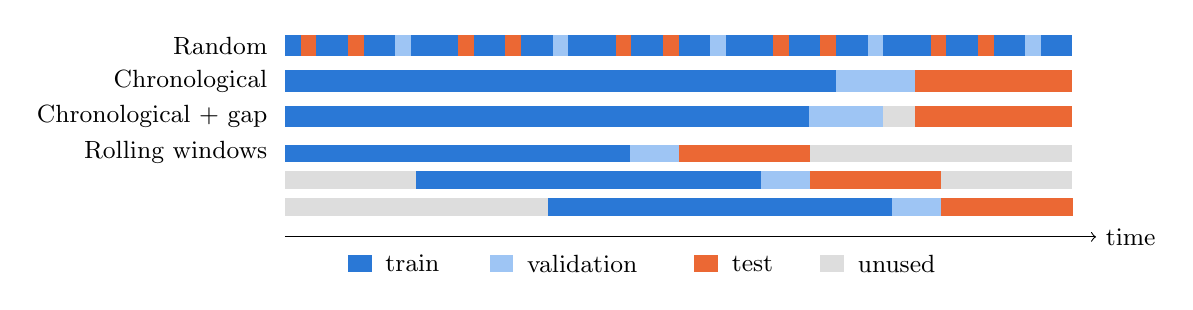
\begin{tikzpicture}[x=0.1cm,y=0.45cm,font=\small]
  \definecolor{tr}{HTML}{2A78D6}
  \definecolor{va}{HTML}{9EC5F4}
  \definecolor{te}{HTML}{EB6834}
  \definecolor{un}{HTML}{DDDDDD}
  % random: interleaved
  \node[anchor=east] at (-1,5.3) {Random};
  \foreach \i in {0,...,49} {
    \pgfmathsetmacro{\r}{mod(\i*7+3,10)}
    \pgfmathparse{\r<2 ? "te" : (\r<3 ? "va" : "tr")}
    \edef\c{\pgfmathresult}
    \fill[\c] (\i*2,5) rectangle ++(2,0.6);
  }
  % chronological
  \node[anchor=east] at (-1,4.3) {Chronological};
  \fill[tr] (0,4) rectangle (70,4.6); \fill[va] (70,4) rectangle (80,4.6); \fill[te] (80,4) rectangle (100,4.6);
  % gap
  \node[anchor=east] at (-1,3.3) {Chronological + gap};
  \fill[tr] (0,3) rectangle (66.5,3.6); \fill[va] (66.5,3) rectangle (76,3.6);
  \fill[un] (76,3) rectangle (80,3.6); \fill[te] (80,3) rectangle (100,3.6);
  % rolling
  \node[anchor=east] at (-1,2.3) {Rolling windows};
  \foreach \w in {0,1,2} {
    \pgfmathsetmacro{\y}{2-\w*0.75}
    \pgfmathsetmacro{\a}{\w*16.67}
    \fill[un] (0,\y) rectangle (100,\y+0.5);
    \fill[tr] (\a,\y) rectangle (\a+43.75,\y+0.5);
    \fill[va] (\a+43.75,\y) rectangle (\a+50,\y+0.5);
    \fill[te] (\a+50,\y) rectangle (\a+66.67,\y+0.5);
  }
  \draw[->] (0,-0.1) -- (103,-0.1) node[right] {time};
  % legend
  \begin{scope}[shift={(8,-1.1)}]
    \fill[tr] (0,0) rectangle (3,0.5); \node[anchor=west] at (3.5,0.25) {train};
    \fill[va] (18,0) rectangle (21,0.5); \node[anchor=west] at (21.5,0.25) {validation};
    \fill[te] (44,0) rectangle (47,0.5); \node[anchor=west] at (47.5,0.25) {test};
    \fill[un] (60,0) rectangle (63,0.5); \node[anchor=west] at (63.5,0.25) {unused};
  \end{scope}
\end{tikzpicture}
\caption{The split protocols. A random split interleaves training and test transactions in time, whereas the chronological protocols score only transactions that occur after every training transaction.}
\Description{Four horizontal bars over a time axis. In the random split, train, validation and test segments are interleaved. In the chronological split the first 70 percent is train, the next 10 percent validation and the last 20 percent test. The gap variant leaves the week before the test period unused. The rolling variant slides a train, validation and test window forward three times.}
\label{fig:splits}
\end{figure}
